\documentclass[openany]{book}
\input{notes_white}
\usepackage{mathtools}
\usepackage{pgfplots}
\settitle{Biology Lab Manual}
\begin{document}
\title{\Large{\underemphasise{Biophysics - Expt 1}} \\ \vspace{5pt}
\large{To estimate the diffusion coefficient from the blob-diffusion experiment}}
\author{Eklavya Raman \\ \vspace{5pt} er24ms024@iiserkol.ac.in \\ \vspace{5pt}
\and Shrey Patnaik \\ \vspace{5pt} sp24ms174@iiserkol.ac.in \\ \vspace{5pt}}
\date{\today}
\maketitle
\begin{center}
    \textbf{Abstract}
\end{center}
    This experiment aims to estimate the diffusion coefficient by analyzing the spread of a dye blob in a medium over time. We analyze the spread using the Image-J software. The principle of diffusion is based on the random motion of particles from regions of higher concentration to regions of lower concentration, leading to an even distribution over time. By measuring the change in the area of the dye blob at different time intervals, we can calculate the diffusion coefficient using Fick's laws of diffusion.
\subsubsection{Aim}
To estimate the diffusion coefficient from the blob-diffusion experiment.
\subsubsection{Apparatus}
\begin{itemize}
    \item Petri dish
    \item Water and Glycerol
    \item KMnO$_4$ solution
    \item Image-J software
    \item Pipette
\end{itemize}
\subsubsection{Working Principle}
The diffusion of the dye in the medium is governed by Fick's laws of diffusion, which describe how the concentration of a substance changes over time and space. In this experiment, we observe the spread of the KMnO$_4$ dye in a water-glycerol mixture, which creates a gradient that drives the diffusion process. By capturing images at regular intervals and analyzing them with Image-J, we can quantify the diffusion coefficient. The method used to calculate the diffusion coefficient is finding the FWHM (Full Width at Half Maximum) of the dye concentration profile, which provides a measure of how far the dye has spread over time. The diffusion coefficient (D) can be estimated using the relation: 
$$\boxed{D = \frac{\sigma_2^2 - \sigma_1^2}{6(t_2 - t_1)}}$$
where $\sigma_1$ and $\sigma_2$ are the standard deviations of the dye concentration profile at times $t_1$ and $t_2$, respectively.
The FWHM is related to the standard deviation ($\sigma$) of a Gaussian distribution by the formula:
$$\boxed{FWHM = 2\sqrt{2\ln{2}} \cdot \sigma \approx 2.355 \cdot \sigma}$$
\subsubsection{Experimental Procedure}
\begin{enumerate}
    \item Measure and add 10 mL of the given solution in a 60 mm petri dish. 
    \item Dry the bottom and set the petri dish on a flat surface, preferably something which provides contrast, like a white paper. 
    \item Keep two tip-boxes to the side and place your phone or camera so that the centre of the petri dish can be imaged.
    \item Take 5 $\mu$L of the KMnO$_4$ solution in a pipette and place a drop at the centre of the petri dish. 
    \item Capture a video of the KMnO$_4$ drop diffusing in the solution.
    \item Stop the video capture when the purple colour has spread to a significant portion of the petri dish, say half of the dish.
    \item Calibrate the camera by placing a ruler in the frame and measuring the distance in pixels corresponding to a known length (e.g., 1 cm).
    \item Analyze the video using Image-J to extract the diffusion data.
\end{enumerate}
\subsubsection{Analysis using Image-J}
\begin{enumerate}
    \item Open the video file in Image-J.
    \item Extract snapshots at relevant time intervals, noting the time stamp, precise to the second at minimum.
    \item Use the red channel to analyze the images. 
    \item Draw an ROI across the center of the dye blob.
    \item Apply the same ROI to the other time point. 
    \item Get the intensity profile of the dye blob at each time point using the "Plot Profile" function.
    \item From the profile, get the maxima, half maxima, and the FWHM.
    \item From FWHM, calculate $\sigma$ using the relation mentioned above.
    \item Use calibration to convert from pixels to cm.
    \item Calculate Diffusion Constant D using the method mentioned above.
    \item Report the findings, including any sources of error and potential improvements for future experiments.
\end{enumerate}
\subsubsection{Observations and Results}
\textbf{KMnO$_4$ in Water-Glycerol Mixture - Eklavya: } \\
\begin{figure}[H]
    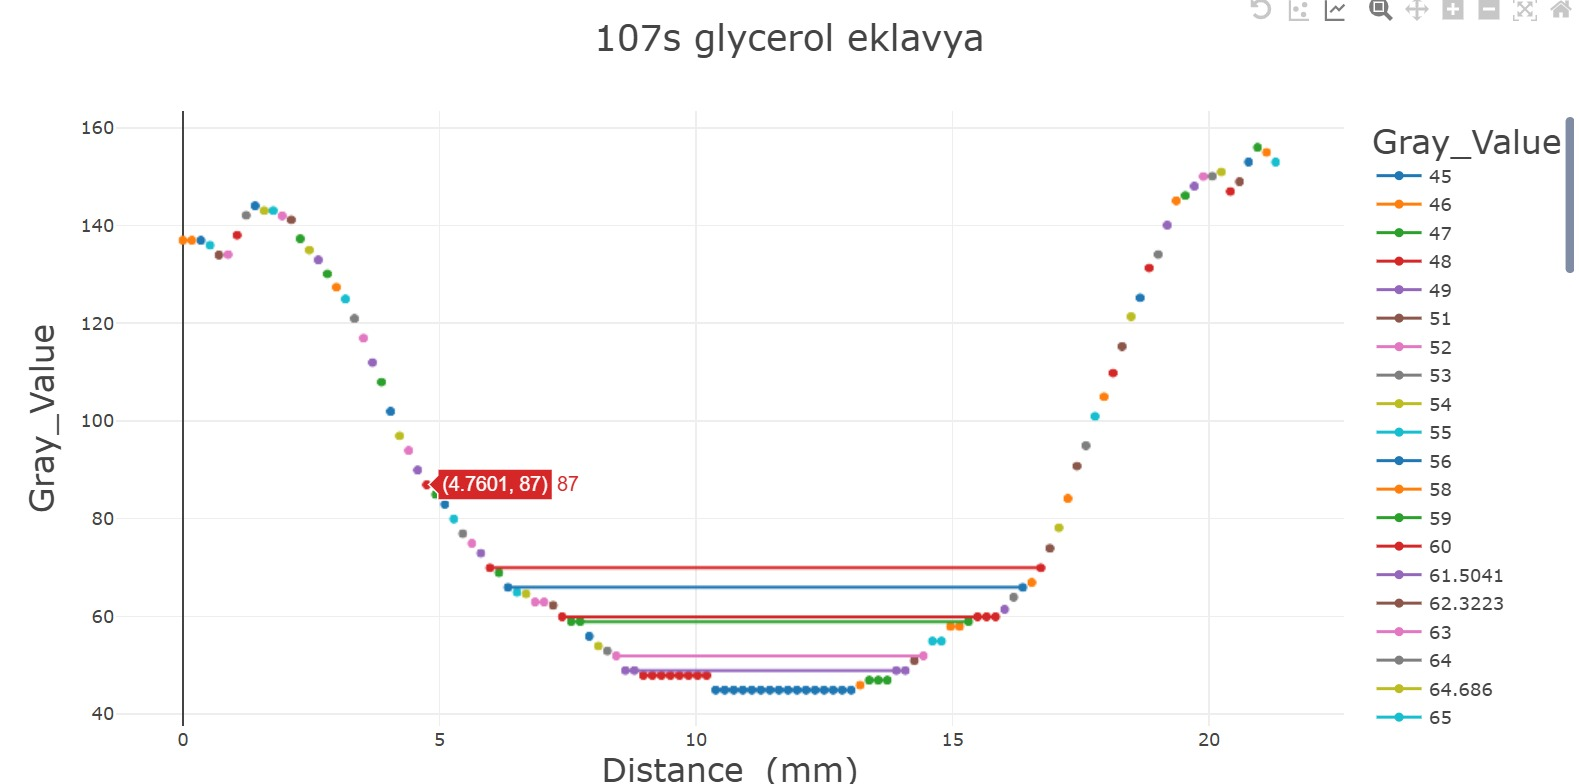
\includegraphics[width=0.5\textwidth]{images/107sEklavyaGlycX1.jpg}
    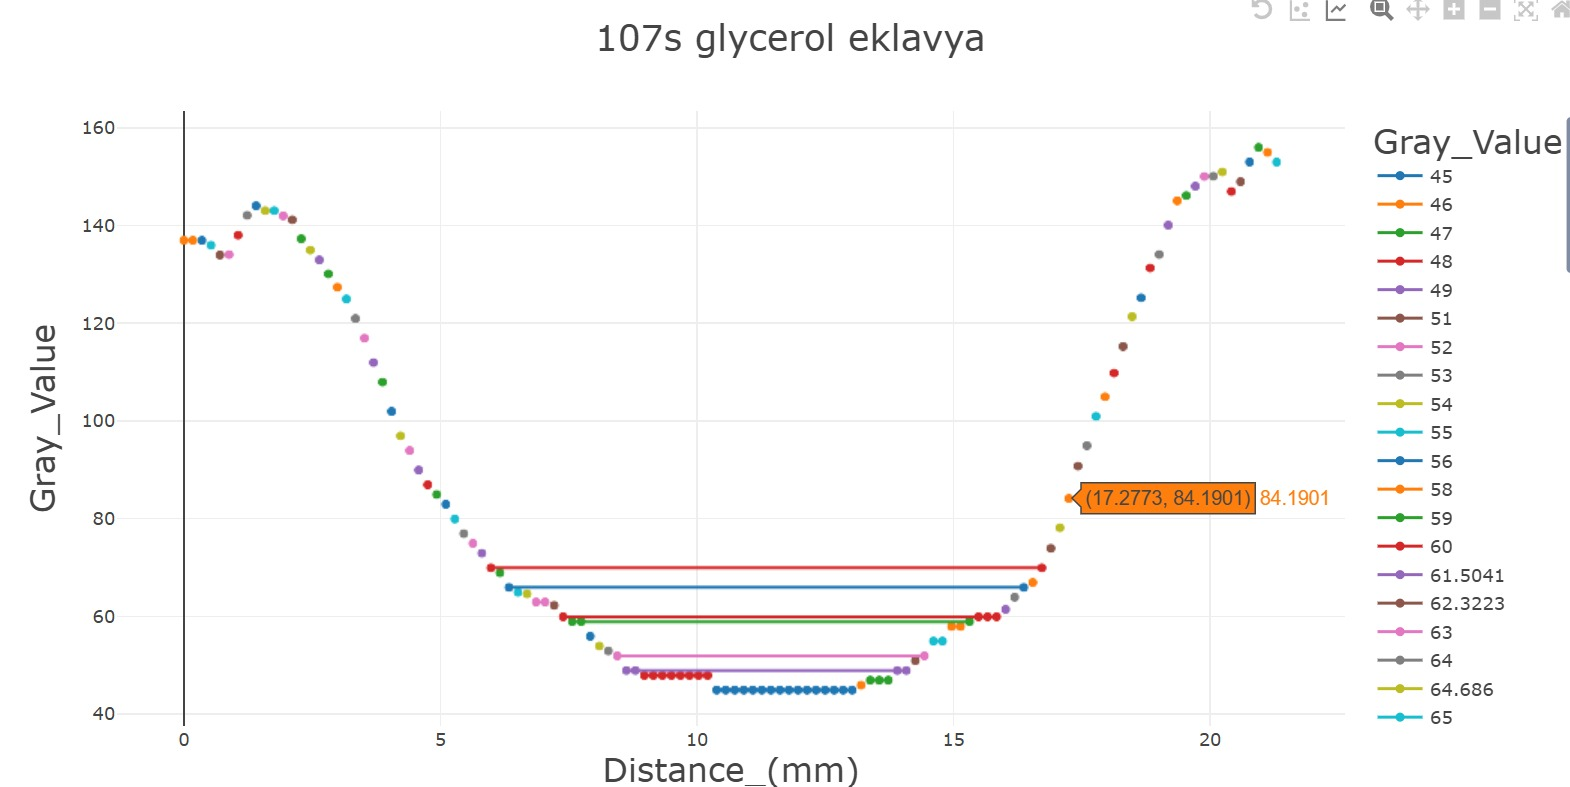
\includegraphics[width=0.5\textwidth]{images/107sEklavyaGlycX2.jpg}
    \caption{Graph of Intensity Profile of KMnO$_4$ in Water-Glycerol Mixture at 107s}
\end{figure}
\begin{figure}[H]
    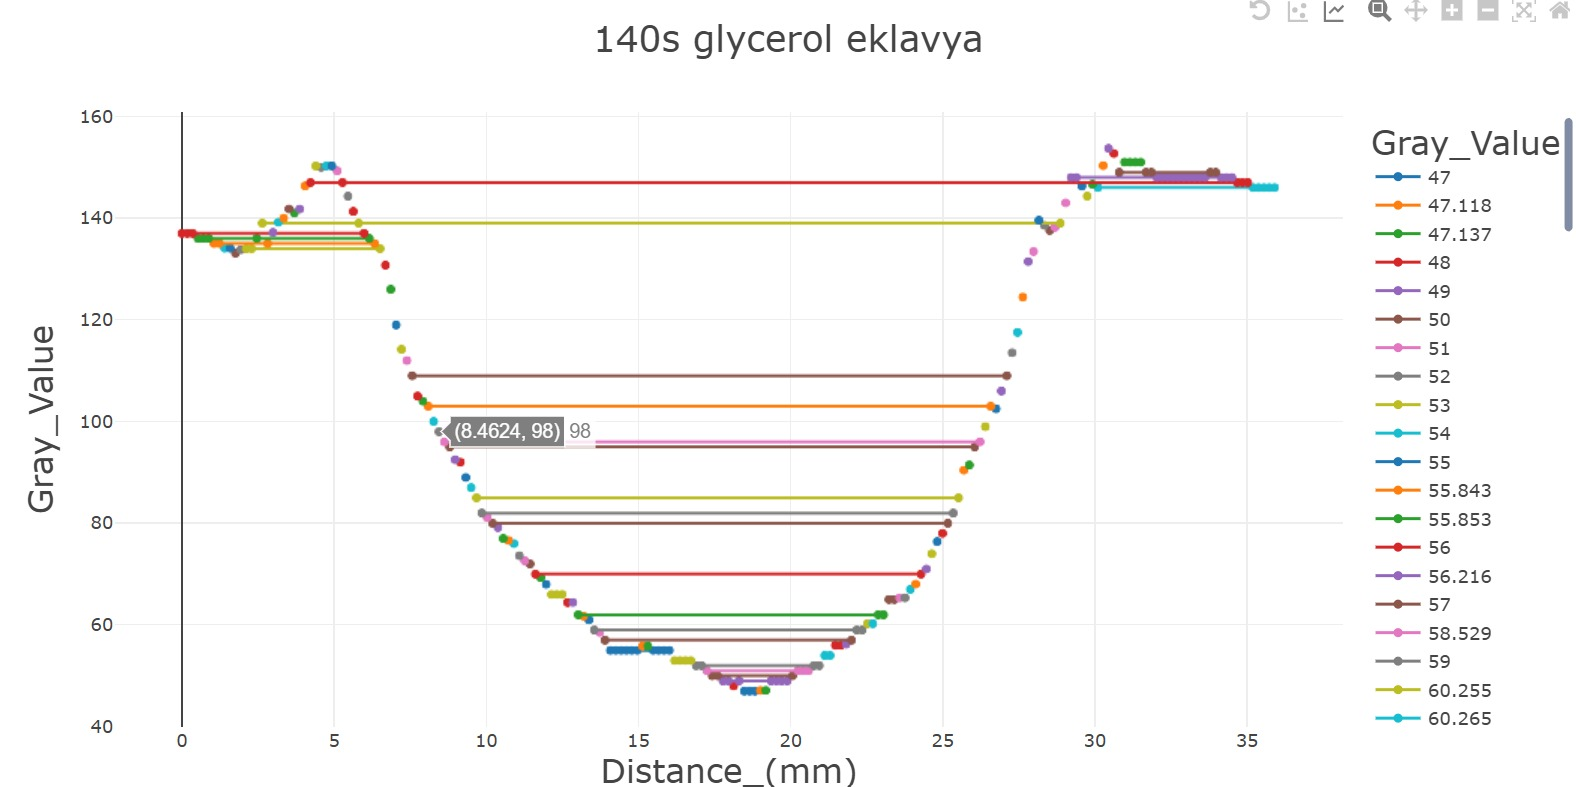
\includegraphics[width=0.5\textwidth]{images/140sEklavyaGlycX1.jpg}
    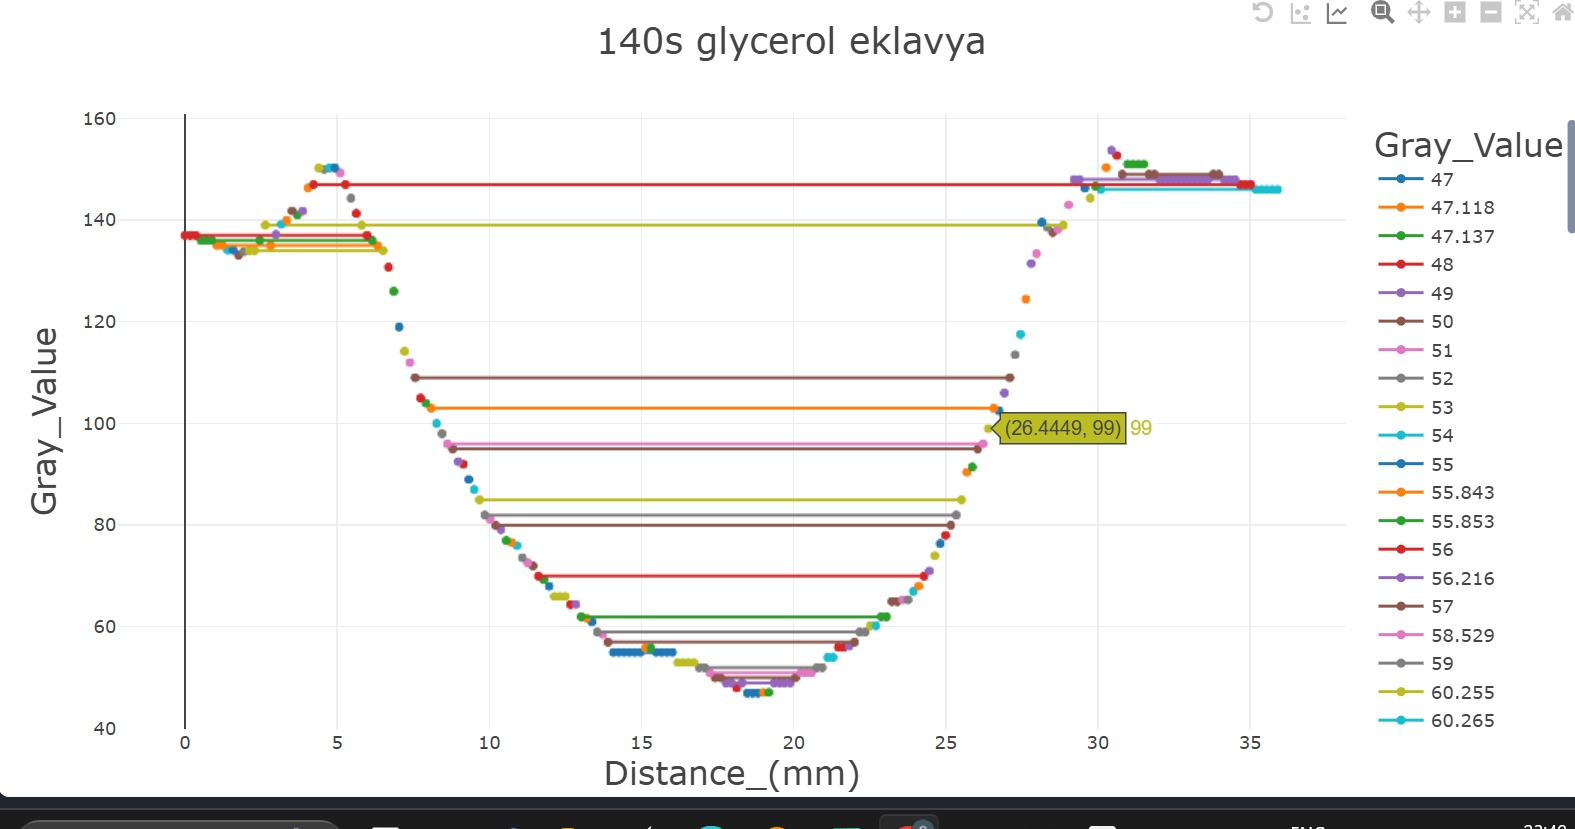
\includegraphics[width=0.5\textwidth]{images/140sEklavyaGlycX2.jpg}
    \caption{Graph of Intensity Profile of KMnO$_4$ in Water-Glycerol Mixture at 140s}
\end{figure}
We have - 
$$\sigma_1 = \frac{FWHM_1}{2.355} = \frac{17.27 - 4.76}{2.355} = 5.31$$
$$\sigma_2 = \frac{FWHM_2}{2.355} = \frac{26.44 - 8.46}{2.355} = 7.63$$
$$D = \frac{\sigma_2^2 - \sigma_1^2}{6(t_2 - t_1)} = \frac{7.63^2 - 5.31^2}{6(140 - 107)} = \frac{58.22 - 28.20}{6(33)} = \frac{30.02}{198} \approx 0.1515 \text{ mm}^2/\text{s}$$
\textbf{KMnO$_4$ in Water-Glycerol Mixture - Shrey: } \\
\begin{figure}[H]
    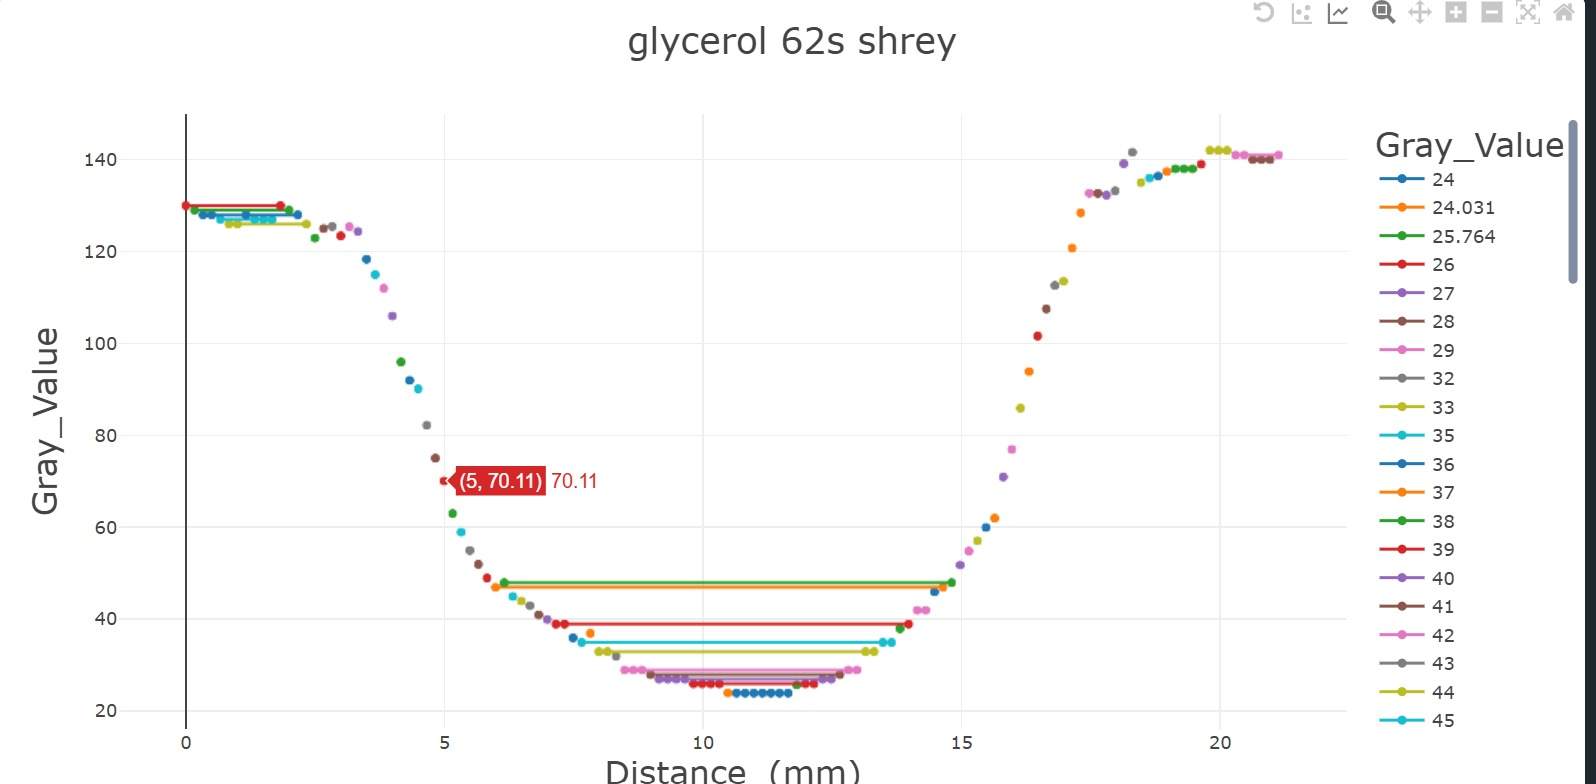
\includegraphics[width=0.5\textwidth]{images/62sShreyGlycX1.jpg}
    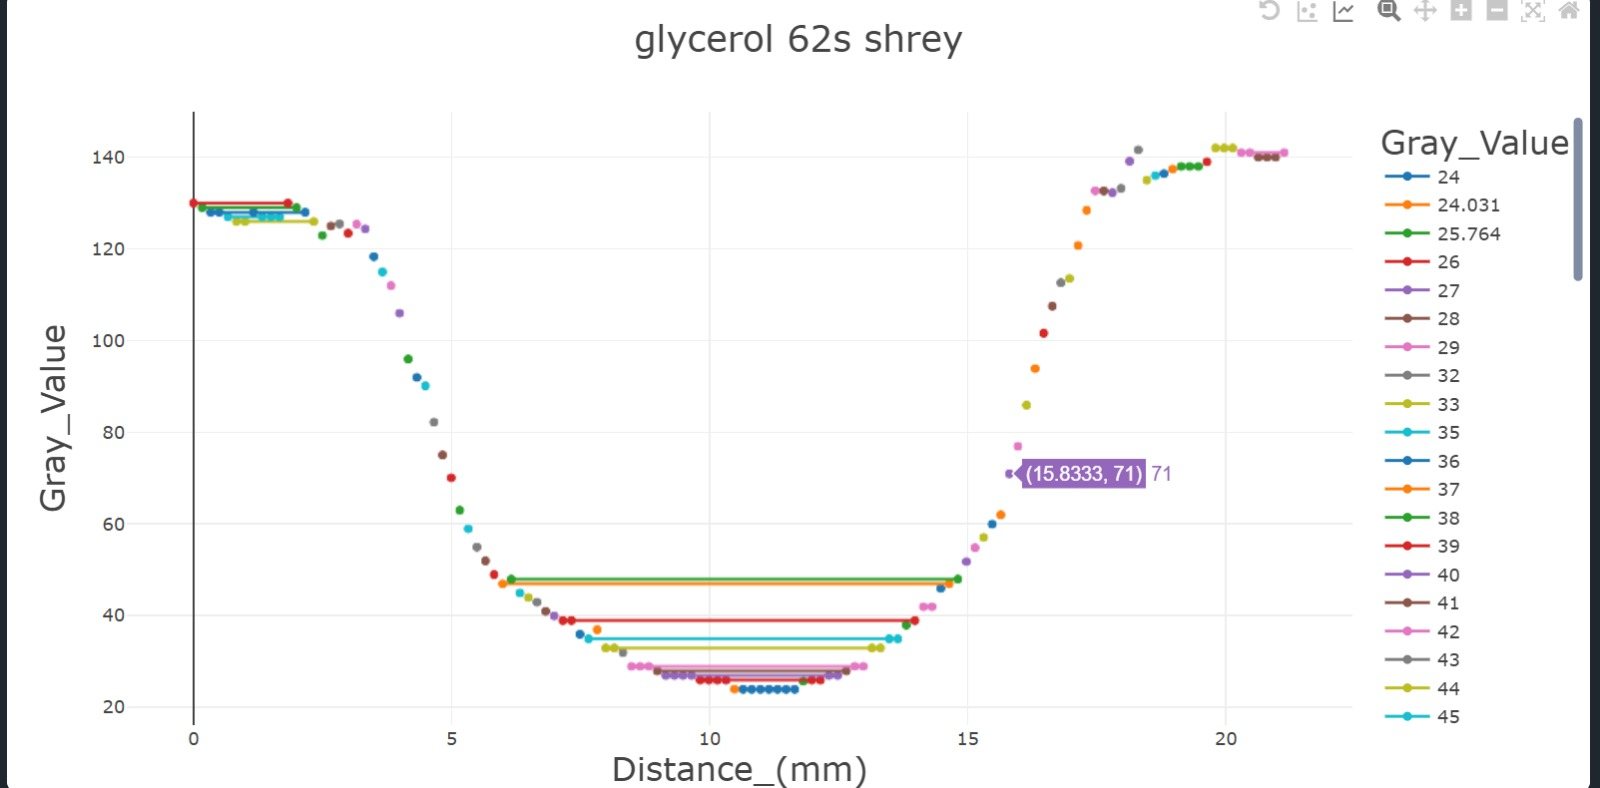
\includegraphics[width=0.5\textwidth]{images/62sShreyGlycX2.jpg}
    \caption{Graph of Intensity Profile of KMnO$_4$ in Water-Glycerol Mixture at 62s}
\end{figure}
\begin{figure}[H]
    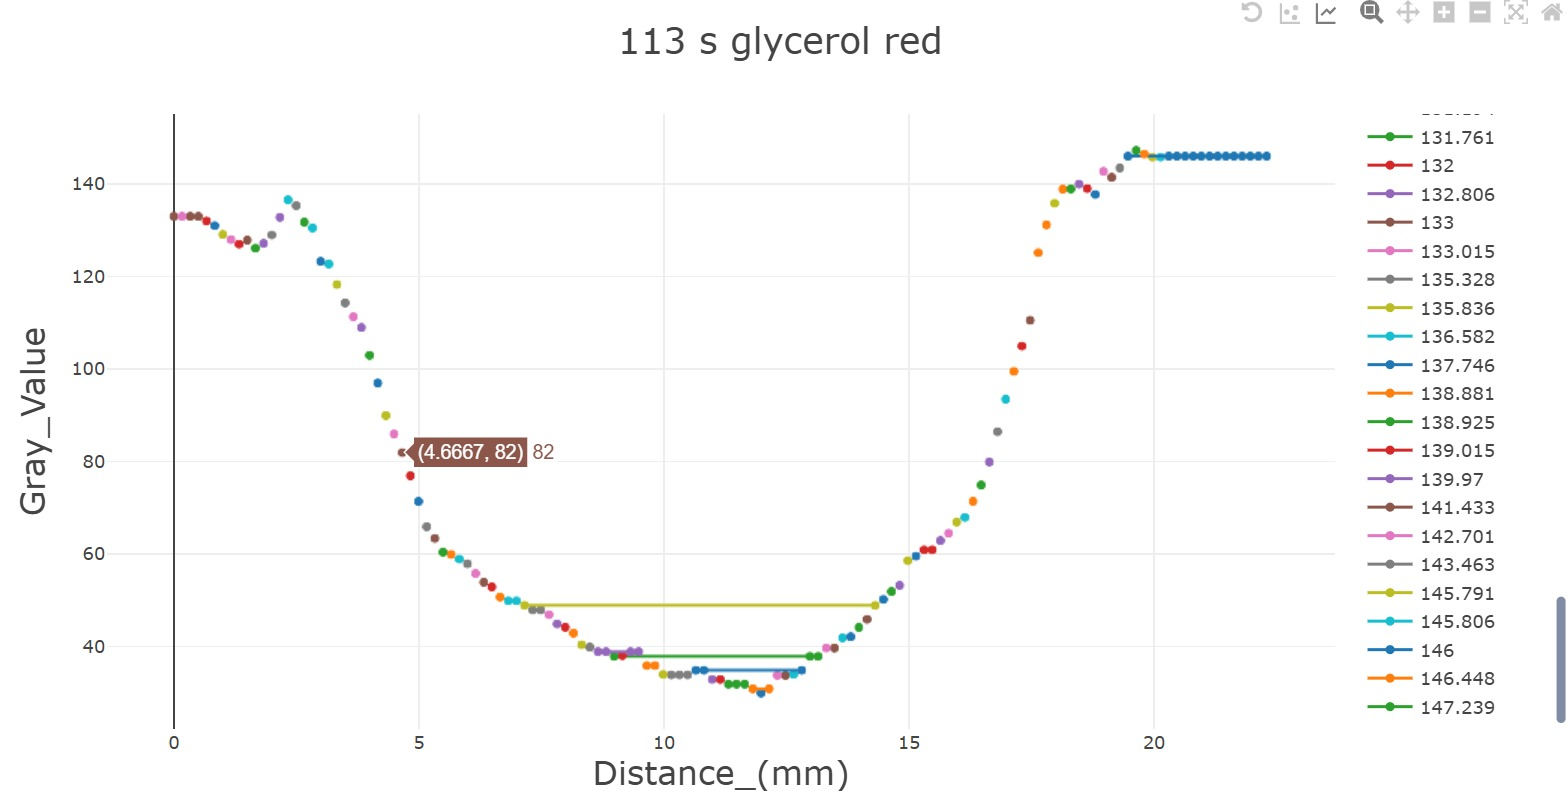
\includegraphics[width=0.5\textwidth]{images/113sShreyGlycX1.jpg}
    \includegraphics[width=0.5\textwidth]{images/113sShreyGlycX2.jpg}
    \caption{Graph of Intensity Profile of KMnO$_4$ in Water-Glycerol Mixture at 113s}
\end{figure}
We have -
$$\sigma_1 = \frac{FWHM_1}{2.355} = \frac{15.83 - 5.7}{2.355} = 4.3$$
$$\sigma_2 = \frac{FWHM_2}{2.355} = \frac{16.66 - 4.66}{2.355} = 5.1$$
$$D = \frac{\sigma_2^2 - \sigma_1^2}{6(t_2 - t_1)} = \frac{5.1^2 - 4.3^2}{6(140 - 107)} = \frac{26.01 - 18.49}{6(51)} = \frac{7.52}{306} \approx 0.02 \text{ mm}^2/\text{s}$$

\textbf{KMnO$_4$ in Water - Eklavya: } \\
\begin{figure}[H]
    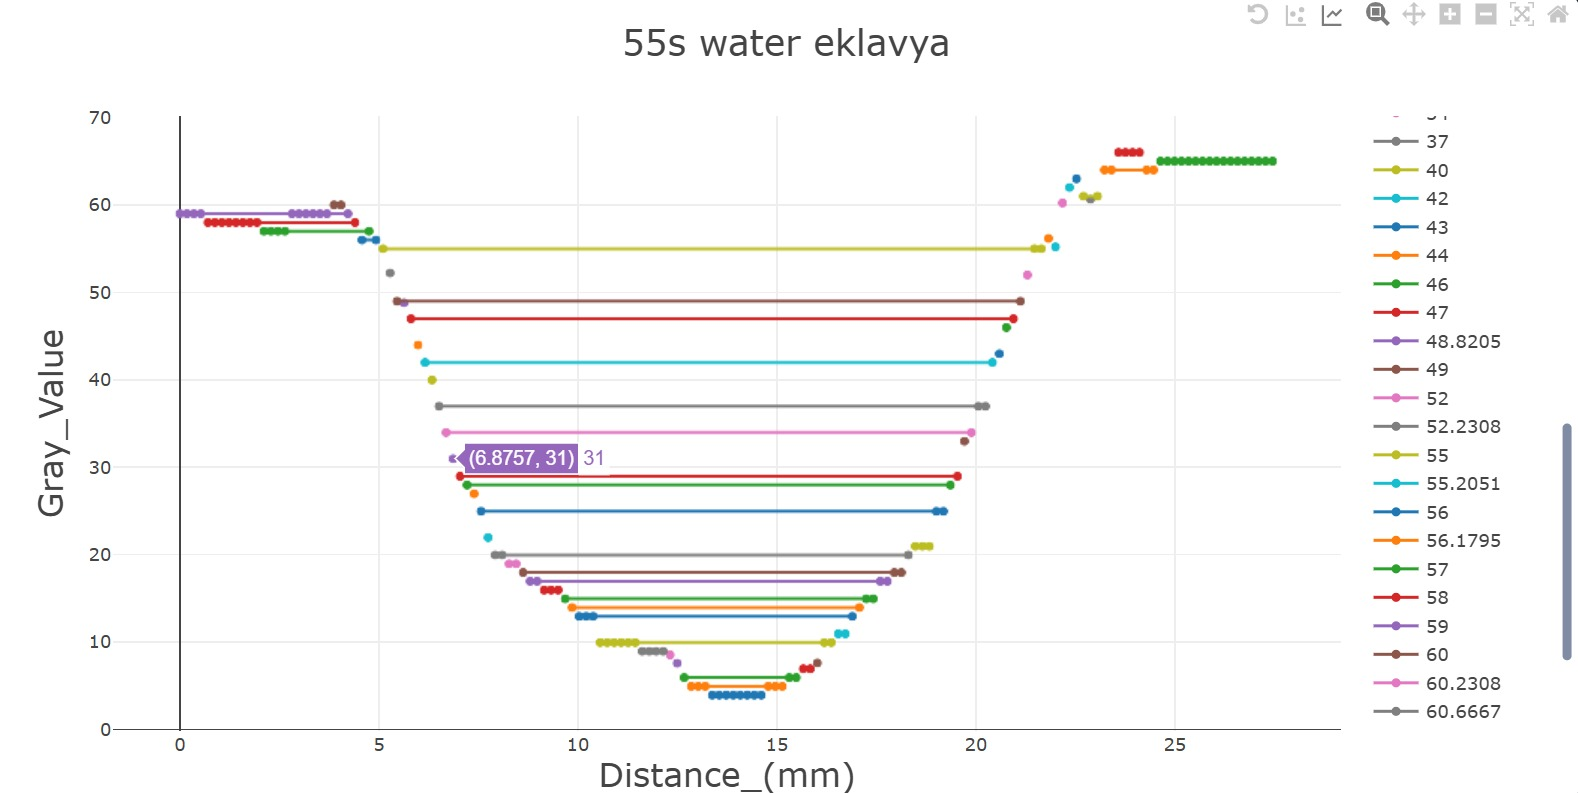
\includegraphics[width=0.5\textwidth]{images/55sEklavyaWaterX1.jpg}
    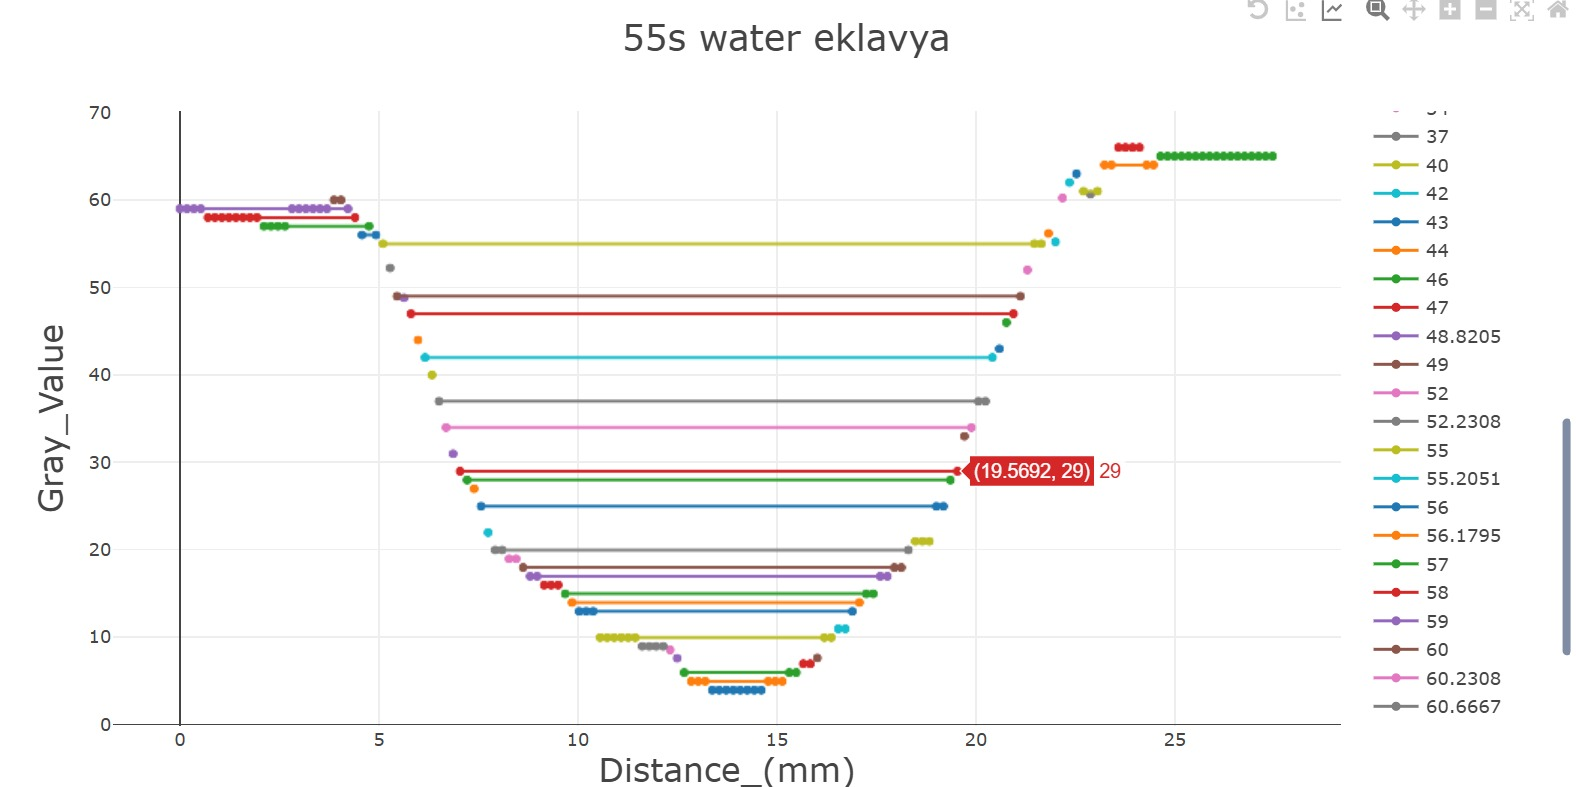
\includegraphics[width=0.5\textwidth]{images/55sEklavyaWaterX2.jpg}
    \caption{Graph of Intensity Profile of KMnO$_4$ in Water at 55s}
\end{figure}
\begin{figure}[H]
    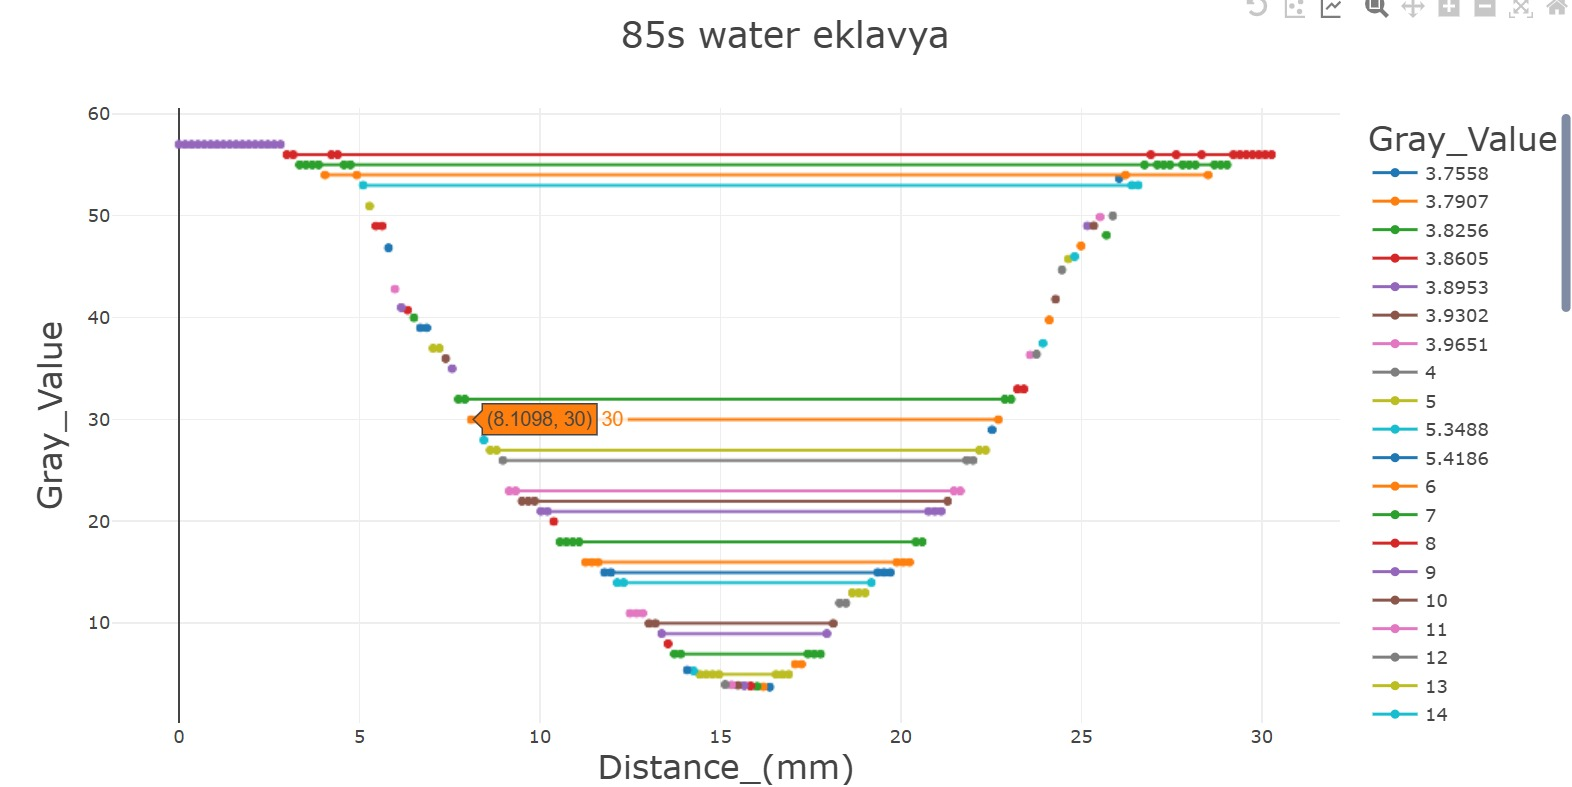
\includegraphics[width=0.5\textwidth]{images/85sEklavyaWaterX1.jpg}
    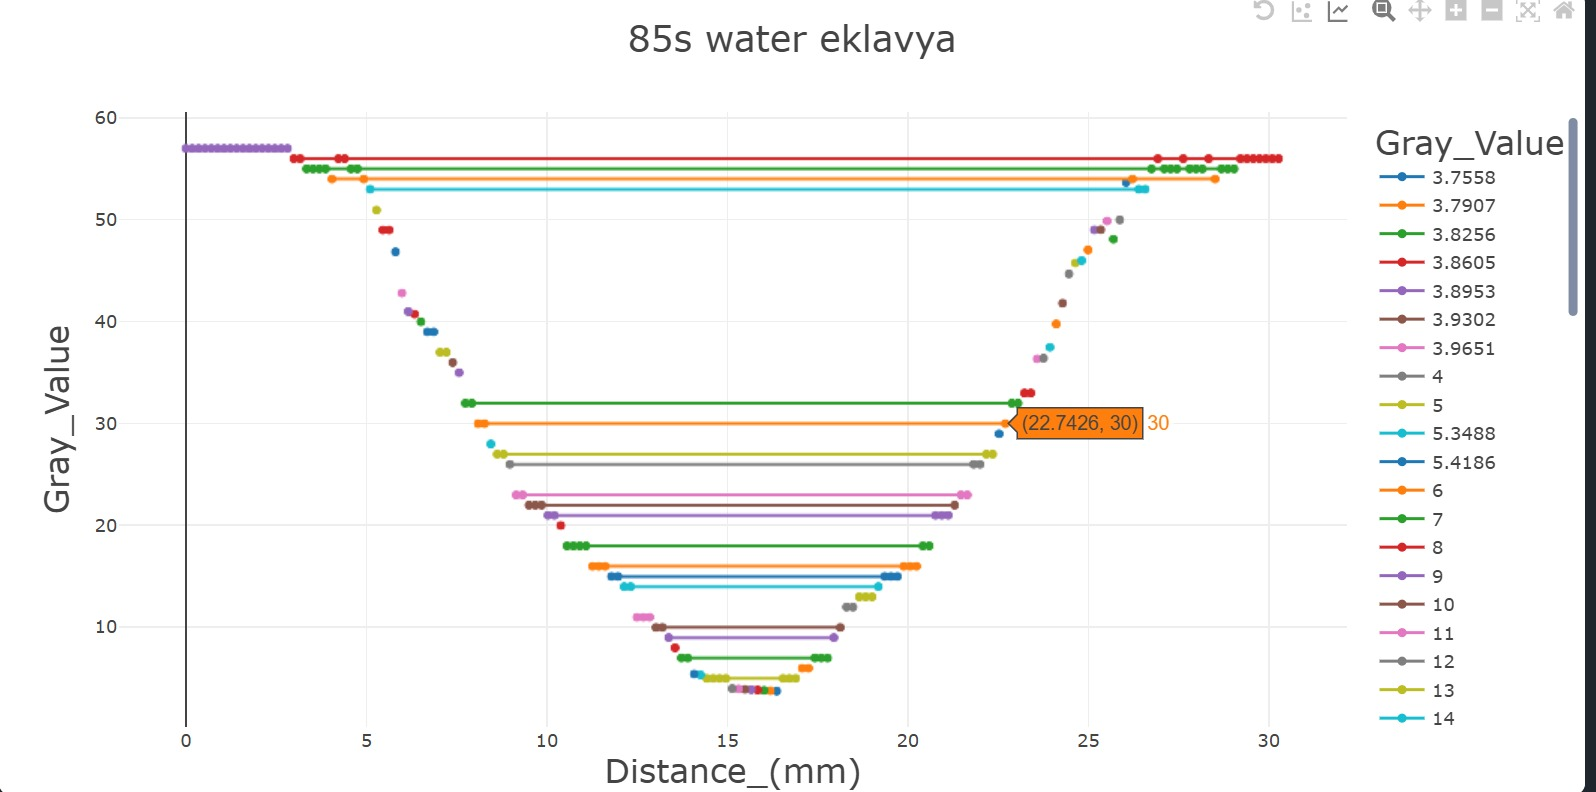
\includegraphics[width=0.5\textwidth]{images/85sEklavyaWaterX2.jpg}
    \caption{Graph of Intensity Profile of KMnO$_4$ in Water at 85s}
\end{figure}
We have -
$$\sigma_1 = \frac{FWHM_1}{2.355} = \frac{19.56-6.87}{2.355} = 5.38$$
$$\sigma_2 = \frac{FWHM_2}{2.355} = \frac{22.75-8.1}{2.355} = 6.22$$
$$D = \frac{\sigma_2^2 - \sigma_1^2}{6(t_2 - t_1)} = \frac{6.22^2 - 5.38^2}{6(85 - 55)} = \frac{38.69 - 28.94}{6(30)} = \frac{9.75}{180} \approx 0.0542 \text{ mm}^2/\text{s}$$
\textbf{KMnO$_4$ in Water - Shrey: } \\
\begin{figure}[H]
    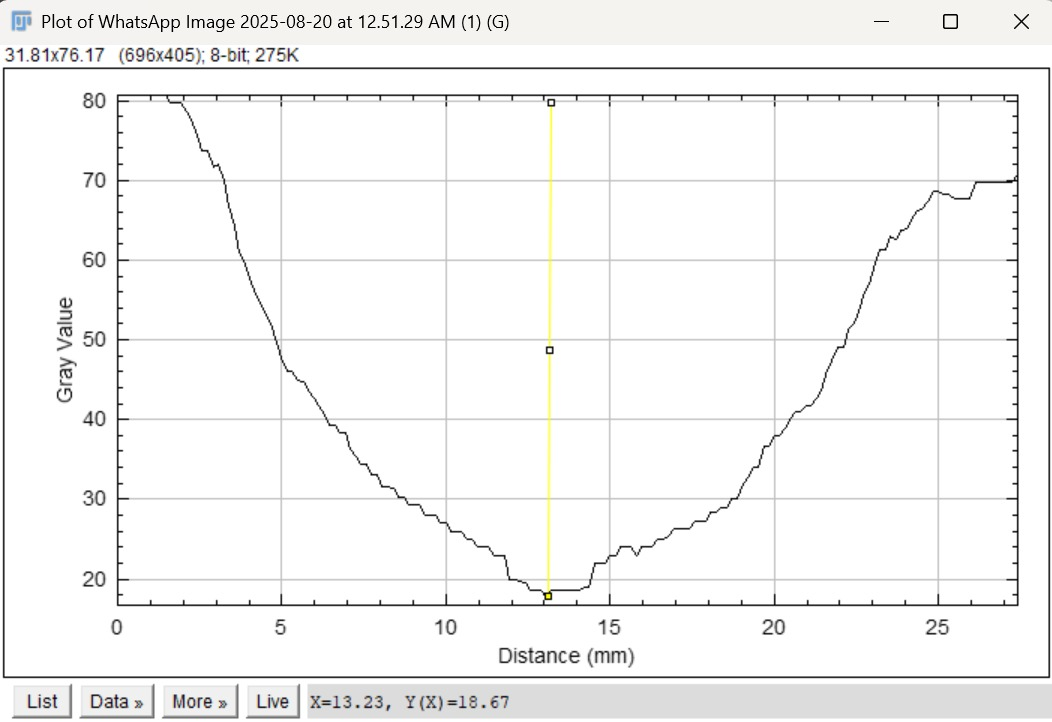
\includegraphics[width=0.5\textwidth]{images/90sShreyWater.jpg}
    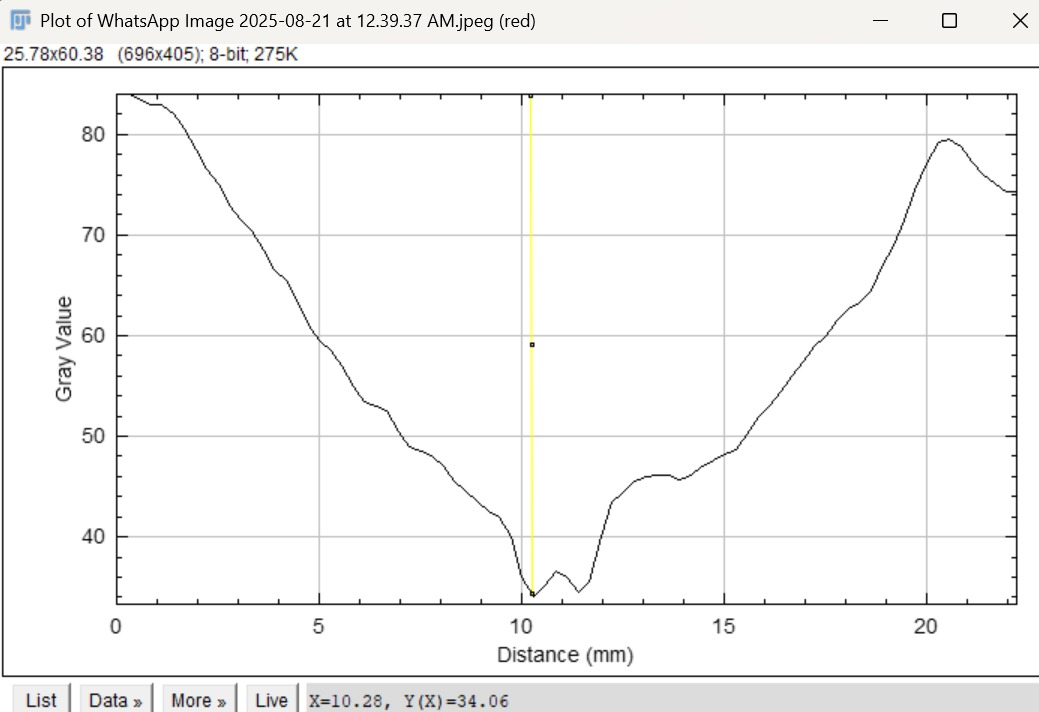
\includegraphics[width=0.5\textwidth]{images/120sWaterShrey.jpg}
    \caption{Graph of Intensity Profile of KMnO$_4$ in Water at 90s and 120s}
\end{figure}
We have -
$$\sigma_1 = \frac{FWHM_1}{2.355} = \frac{22.0 - 5.0}{2.355} = 7.21$$
$$\sigma_2 = \frac{FWHM_2}{2.355} = \frac{17-5}{2.355} = 5.09$$
$$D = \frac{\sigma_2^2 - \sigma_1^2}{6(t_2 - t_1)} = \frac{7.21^2 - 5.09^2}{6(120 - 90)} = \frac{51.98 - 25.90}{6(30)} = \frac{26.08}{180} \approx 0.144 \text{ mm}^2/\text{s}$$
\subsubsection{Conclusion}
The diffusion coefficients for KMnO$_4$ in different media were estimated using the blob-diffusion experiment and analysis with Image-J software. The calculated diffusion coefficients are as follows:
\begin{itemize}
    \item KMnO$_4$ in Water-Glycerol Mixture - Eklavya: $D \approx 0.1515 \text{ mm}^2/\text{s}$
    \item KMnO$_4$ in Water-Glycerol Mixture - Shrey: $D \approx 0.02 \text{ mm}^2/\text{s}$
    \item KMnO$_4$ in Water - Eklavya: $D \approx 0.0542 \text{ mm}^2/\text{s}$
    \item KMnO$_4$ in Water - Shrey: $D \approx 0.144 \text{ mm}^2/\text{s}$
\end{itemize}

\end{document}